% @author Marcel Ruland (2018)
%
%% Random pieces of information I picked up along the way (might turn out useful)
% [chapterprefix=true] changes ``1 LaTeX'' to ``Chapter 1\\ LaTeX''

%% tell TeXshop to compile using LuaLaTeX and encode with UTF-8
%!TEX TS-program = lualatex
%!TEX encoding = UTF-8 Unicode

\documentclass[
	fontsize=11,			% font size 10pt
	paper=11.8cm:15.8cm,	% tolino Epos screen dimensions
	DIV=15,					% KOMA calculates Satzspiegel
	pagesize,				% ensures compatibility with PDF and DVI
	toc=bib,				% include bib in toc
	toc=listof,				% include list of tables and list of figures in toc
	abstract=true,			% display abstract heading
	titlepage=firstiscover,	% set title page as cover page
	footnotes=multiple,		% separate footnotes set directly one after another by a comma
	headinclude,
]{scrreprt}

\usepackage{ba_style_ereader}  % loading packages, typesetting, etc.


% using all commands now to have an exhaustive list and see what they're all doing, will probably remove some of them at some stage
%\titlehead{Titlehead}
\subject{%
Universität Paderborn \\[0.5em]
Fakultät für Kulturwissenschaften \\
Fakultät für Elektrotechnik, Informatik und Mathematik
}
\title{Applying Frequent Pattern Mining to Multimodal Behaviour in Interaction}
\subtitle{Visualising Significant Patterns}
\author{\addfontfeature{Style=Alternate} Marcel Ruland}
\date{Hand-in date: \today}
\publishers{%
	supervised by \\
	Prof.~Dr.~Katharina Rohlfing \\
	Prof.~Dr.~Eyke Hüllermeier
}
\begin{document}
\maketitle
%% !TEX root = ../ba_scrreprt_master.tex
% @author Marcel Ruland (2018)

\begin{abstract}  % @author Katharina Rohlfing (2018)
Human social interaction can be characterised by multimodal behaviour.
According to theoretical positions emphasising that communication is organised by the interaction partners jointly, we identified the challenge of assessing human sequential behaviour that is spread across different modalities and co-constructed with a partner.
In previous work, we faced this challenge by applying frequent pattern mining in an analysis of a corpus of mother-child dyads.

The application of frequent pattern mining provided some support and initial results for the proposition that human interactive behaviour is sequentially organised.
Accordingly, verbal and nonverbal behaviour are co-constructed by the interaction partners and form a range of patterns.
For example, with respect to the occurrence of maternal vocal behaviour, some nonverbal framing was notable.
Firstly, one pattern with a high confidence suggests an intrapersonal sequence of gazing at the infant, smiling, and speaking.
In contrast, another pattern suggests an interpersonal sequence of mother gazing at her infant, infant gazing back, followed by vocal behaviour of the mother.
The analysis reveals patterns emerging between infants as young as 3-months-old and their mothers.

Taken together, frequent pattern mining is a more exploratory analysis as the premises and conclusions emerge as a result of it.
While this method yields contingencies and dependencies and provides their frequencies, it is not yet investigated how the significance of these patterns can be calculated for behavioural studies and how it can be visualised.
Our paper presents first solutions to the problem of how to discern and visualise the significance of some patterns with respect to other existing patterns in the sample.
\end{abstract}
\tableofcontents

% !TEX root = ../scrreprt_light/ba_light_master.tex
% @author Marcel Ruland (2018)

\chapter{\introduction}
\label{ch:intro}
A \emph{turn} is a basic unit of speech in conversation.
When a speaker begins their turn, they gain the right to speak and\dash upon finishing their utterance\dash pass that right on to another participant of the conversation.
A turn is on average 2~\s\ in length, with very high variation.
It usually consists of syntactically complete clauses and gives pragmatically sufficient information, though this is not a necessity \citep[\pnum{8}]{levinson_turn-taking_2016}.
\emph{Turn-taking} is the act of one speaker finishing their turn and another speaker beginning their turn, i.e.\ passing on the right to speak from one speaker to another. % Anke's diagram here?
Turns and turn-taking must not necessarily be strictly linguistic (in the sense of making use of language only, without other modalities playing relevant roles), but may make use of, for example, gestures \citep[\pnum{28--43}]{schmitt_zur_2005}.
In fact, children regularly engage in turn-taking before having acquired their first words \citep[\pnum{1311}]{casillas_turn-taking_2016}.
Turn-taking is therefore not intrinsically linguistic in and of itself.

If turn-taking is not dependant on the linguistic modality but may make use of it, then it logically follows that turn-taking must be a multimodal phenomenon.\footnote{%
Assuming there is no such thing as non-modal turn-taking.}
Despite this fact, turn-taking has so far mostly been considered as unimodal in the literature \citep[\pnum{1}]{rohlfing_multimodal_underreview}.
The downside of investigating only one modality of a multimodal phenomenon is\dash quite obviously\dash that it ``omits other behaviors relevant to the exchange'' \citep[\pnum{3}]{rohlfing_multimodal_underreview}.

\citet{rohlfing_multimodal_underreview} have identified and approached turn-taking as a multimodal phenomenon; taking into consideration linguistic utterances, non-linguistic vocalisations, gaze, and smile.
They did so by applying \fpmlower, a technique at the intersection of statistics and computer science, to a corpus of 10 mother-infant dyads.
The fundamental aim of \fpmlower\ is to find patterns in a data set that occur \emph{frequently}.
The specific kind of pattern and the definition of \emph{frequent} cannot be meaningfully generalised and depend heavily on the individual application.
In contrast to descriptive and inferential statistics\dash which disprove or affirm hypotheses generated beforehand\dash \fpmlower\ is of an exploratory, hypothesis-generating nature.
Depending on the patterns found, one may then formulate hypotheses based on these found patterns, which may then in turn be tested empirically using descriptive and inferential statistics \cite[\pnum{6~ff.,~tba}]{rohlfing_multimodal_underreview,han_data_2012}. %% ISSUE: How do you give page references for each individual source when citing multiple sources?
The basic concepts of \fpmlower\ are explained by \citet[\pnum{57}, emphasis in original]{han_frequent_2007}:
\begin{quote}
``Frequent patterns are itemsets, subsequences, or substructures that appear in a data set with frequency no less than a user-specified threshold.
For example, a set of items, such as milk and bread, that appear frequently together in a transaction data set, is a \emph{frequent itemset}.
A subsequence, such as buying first a PC, then a digital camera, and then a memory card, if it occurs frequently in a shopping history database, is a \emph{(frequent) sequential pattern.}''
\end{quote}

The present thesis aims to strengthen the statistical objectiveness of applying \fpmlower\ to human interaction by introducing a notion of significance.
It is organised into five main chapters.
Chapter \ref{ch:intro} (i.e.\ the current chapter) will proceed by GOD KNOWS WHAT.
The second chapter explains the entire process of preparing the data, applying \fpmlower, and then evaluating the data\dash beginning with a description of the raw video material and ending with abstract rules\footnote{The notion of a \emph{rule} will be explained in subsection \ref{ssec:miningmethodapproach}.}.
Chapter \ref{ch:significance} introduces a method for establishing statistical significance in the data.
Both chapter \ref{ch:mining} and \ref{ch:significance} present results in their last sections.
Chapter \ref{ch:visualisation} is of a different nature.
In contrast to the two previous chapters, it is not concerned with methods of evaluating the data but with methods of making the results easily comprehensible for humans by visualising them in an adequate way.
Finally, chapter \ref{ch:conclusion} concludes the thesis.




\section{Why is Turn-Taking important?}
\label{sec:intrott}
According to present knowledge, turn-taking is a universal feature of human language, a \emph{language universal.}
A language that does not make use of turn-taking has not been found to date and it is unlikely that such a language will ever be found (although\dash as is always the case in empirical science\dash this is not impossible).
Its implications to language processing and production are fundamental as it dictates the temporal organisation of the flow of information between humans.
Turn-taking may be characterised as a temporal phenomenon.
Its temporal structure shows high variation in length of individual turns, which average at 2~seconds \citep[\pnum{7}]{levinson_turn-taking_2016}, but little variation in the gaps between turns, whose modal length in American English telephone conversations is 200~\ms\ \citep[\pnum{16}]{levinson_timing_2015}.

Zooming out, turn-taking is not only present in humans.
Figure \ref{fig:species}, based on \citet[\fnum{2}]{levinson_turn-taking_2016}, shows a number of related species who are known to employ either vocal or gestural turn-taking.
The original purpose of \citeauthor{levinson_turn-taking_2016}'s figure was to show the presence of turn-taking in non-human primates, it can therefore not be considered exhaustive.
I have added \emph{diaemus youngi}, one of several bat species known to engage in vocal turn-taking \citep[\pnum{114}]{vernes_what_2017}, to show that the phenomenon is in fact further spread in the animal kingdom than the various apes and monkeys might lead one to believe.
Some indications for turn-taking have also been found in European starlings, which have been shown to at least prefer song alternation to song overlap \citep{henry_social_2015}, and there are many more examples.
\citet[\pnum{6}]{levinson_turn-taking_2016} suggests that language followed turn-taking in evolution. He does not consider this a coincidence but furthermore suggests that turn-taking formed the basis for language evolution.
This claim rests on three main indications: a) turn-taking is present in various species related to humans, b) humans commonly employ language together with other modalities present in various non-human primates (e.g.~gesture), and c) language development in infants begins at an early age.

Taking another step back, this raises the question of how turn-taking itself was selected for in evolution.
From this point of view, turn-taking is more interesting than other language universals, whose evolutionary advantages are quite obvious.
The notion of a subject or the notion of a verb \citep[both considered language universals,][]{robins_noun_1952,hopper_iconicity_1985} allow humans to express a variety of semantic concepts that they may not be able to express without these notions.
The evolutionary advantage of turn-taking, on the other hand, still remains unclear.
Fundamentally, evolution works by means of random mutations in the passing on of an organism's \dna.
The \dna\ of the first child generation entirely depends on the \dna\ of the parent generation\dash with occasional random mutations introduced \citep[\cnum{8}]{dediu_introduction_2015}.
On a non-genetic level, one might rephrase this by stating that, with every new generation, organisms do not make exact copies of themselves, but copies with ever so slight modifications \citep[\cnum{8}]{dediu_introduction_2015}.
This mechanism is what Charles Darwin referred to as ``descent with modification'' \citep[\pnum{116}]{darwin_origin_1958}.
These modifications may result in all sorts of differences between a parent and their child.
Be it less muscle mass, a lighter feather colour, or a more sophisticated sense of hearing.
Naturally, as these modifications are random, they will cancel each other out in the larger picture.
For every bat born with thinner wings, there will be another one with thicker wings; for every human with more red blood cells, there will be another one with fewer red blood cells; and so on.
The only circumstance under which a change can permanently push through in the long run and become the norm in an entire population is if that new trait causes its bearers to produce significantly more offspring than those individuals who do not bear the trait.
As a result of the significantly higher offspring, the new trait will be present in significantly more individuals in the first child generation, who in turn will pass it on to even more individuals of the second child generation.
Over time, those individuals bearing the trait will outnumber the individuals not bearing the trait until eventually the new trait will be present in all individuals of the species.%
\footnote{This is a rough sketch of a complex process, omitting many details which are less relevant for the issue at hand.
For example, the new trait must have high heredity. This refers to the property of a trait being passed on to a large proportion of the child generation \citep{king_heredity_2013}.
Humans wearing earrings can be fairly certain that their offspring will inherit the property of having two hands.
They can be much less certain that their offspring will also be wearing earrings.
Having two hands is a trait with relatively high heredity; wearing earrings is a trait with relatively low heredity \citep[\pnum{243~ff.}]{sapolsky_behave_2017}.
Furthermore, there are theoretical positions stating that evolution in the sense described here only applies after the percentage of individuals in a population bearing the trait has surpassed a certain threshold.
Below this threshold, the only mechanism at work is chance.
It is also debated whether this threshold is dependant on or independent of the total population size \citep[\pnum{21~f.},\pnum{90--94}]{berwick_why_2016,gillespie_population_2010}.}
This evolutionary advantage is not always straight-forward and easy to spot.
It may be intuitive that a male gorilla with stronger muscles is more successful in a mating battle; much less intuitive that a larger skin surface can take in more warmth from the sun, which is then followed by an easier maintaining of body temperature \emph{(thermoregulation),} leading to better survival in colder climates and consequently more chances of successful mating.
The latter, less intuitive example is a rough sketch of how the first stages of the evolution of wings are hypothesised to have taken place \citep{douglas_thermoregulatory_1981,kingsolver_aerodynamics_1985}.
An implicit necessity of the evolutionary mechanism is that every single evolutionary step along the way must in itself be of use to its bearers.
Sticking with the wing-example, organisms will not develop tiny winglets that become bigger and bigger because somewhere down the line they will become useful for flight.
The initial tiny winglets would never gain a foothold in the population if their bearers were not in advantage.
Every tiny adaptive step in itself must have been useful, be it thermoregulation, aerodynamics, or any other kind of advantage.

How does turn-taking fit in this picture?
Being a characteristic of a communication system, it seems an arbitrary, even counterproductive restriction to impose.
If we think of a communication system between two organisms, the a priori assumption would be that information simultaneously flows from \emph{a} to \emph{b} and from \emph{b} to \emph{a}.
Limiting information flow to only one direction at a time is a considerable disadvantage that must be justified by some other advantage it may be a byproduct of.
Two possible reasons for this restriction come to mind, the first of which unpacks as follows:

If, in a conversation, participant \emph{a} listens to participant \emph{b} and speaks at the same time, then what will in effect reach \emph{a}'s ear is a mixture of both participants' speech.
\emph{a} is now challenged with the task of disentangling the two sources and isolating \emph{b}'s signal from the received input.
Avoiding this difficult task may well be worth limiting information flow to one direction only.
But for several reasons, this does not seem to be the case.
First off, the capacity to isolate a human voice in an environment of several voices is a capacity that to a certain extent is already present in humans.
In psychoacoustics, it is known as the cocktail party effect \citep[first mentioned in][a more recent review is given in \citeauthor{arons_review_1992}, \citeyear{arons_review_1992}]{pollack_cocktail_1957}.
But even if humans were not capable at all of discerning a single voice in a noisy environment, turn-taking still could not be justified by this line of argument. The described scenario of having to separate two acoustic signals from each other is in fact a peculiarity of the acoustic modality.
It is no challenge at all to \emph{see} another conversation partner's gestures while producing gestures at the same time\dash the visual modality allows such simultaneity.
Consequently, this line of argumentation fails for gestural turn-taking.
Motivating gestural and vocal turn-taking differently would tremendously complicate any theory of turn-taking and should therefore be avoided unless the empirical data contain strong clues hinting in such a direction.
As of now, this is not the case and therefore the sensible assumption is that this line of argumentation will also fail as a cause for vocal turn-taking.%
\footnote{
Explained differently:
It is of course true that for the acoustic modality this line of argumentation is not wrong per se.
But it is in all probability not the cause for vocal turn-taking.
Claiming that ``vocal turn-taking is caused by the difficulties of separating two acoustic signals from each other'' is similar to claiming that ``infants decide to stop being breast fed because they cannot survive from nothing but breast milk their entire life''.
It is of course true that breast milk does not contain nutrients suited for an adult human and does not come in quantities sufficient to feed a human their entire life.
But anyone who has ever seen the looks on infants' faces when their parents decide to stop breast feeding knows that this is not a choice the infant approves of.
They stop being breast fed because their parents decide to stop breast feeding them.}
Further support for the claim that this acoustic peculiarity is not responsible for turn-taking is the fact that turn-taking is equally present in sign languages, which make use of the visual modality \citep[see e.g.][among many others]{devos_turn-timing_2015,girard-groeber_management_2015, groeber_turns_2014,manrique_suspending_2015,mcclearly_turn-taking_2013}.

The second possible justification for turn-taking that comes to mind is a competition for resources.
Maybe the human brain is simply not capable of mastering both the production and reception task at the same time.
But again, this cannot be the whole story.
\citet{levinson_timing_2015} analysed the gaps between turns in the Switchboard Corpus, a corpus consisting of American English telephone conversations recorded across the \textsc{usa} \citep{calhoun_nxt-format_2010,godfrey_switchboard_1992}.
They defined a gap, following \citet{heldner_pauses_2010}, as ``portions of the stereo signal that contained silence in each speaker's channel, and that involved a floor transfer between the two speakers'' \citep[\pnum{16}]{levinson_timing_2015}.
This definition is in part unclear because \citet[\pnum{556}]{heldner_pauses_2010} do themselves not define what a \emph{floor transfer} is but merely give the term as one of many in a list of synonyms having been used in the literature\dash all essentially meaning \emph{gap} or \emph{pause}.
However, \citet[\pnum{556}]{heldner_pauses_2010} define a \emph{gap} as ``silences bounded by speech from different speakers'' and it becomes clear from context that this is also the definition \citet{levinson_timing_2015} have in mind.
\citet{levinson_timing_2015} found that the modal gap between turns had a length of only 200~\ms.
In a large meta-analysis of 82 studies on word production, \citet{indefrey_spatial_2004} and \citet{indefrey_spatial_2011} (the latter being a later update in light of recent research advances) state that the production time of a single primed\footnote{%
DEFINITION OF PRIMING}
word is 600~\ms.
Referring to this meta-analysis, \citet{levinson_turn-taking_2016} points out that this minimal production time is already longer than the modal gap of 200~\ms\ found in \citet{levinson_timing_2015}.
Consequently, speech production must begin before the end of the previous turn.
Or, in other words, this is evidence for the fact that at least for a finite amount of time human cognitive resources are sufficient for receiving and planning speech at the same time.
Planning is of course in its cognitive demands not necessarily identical to producing\dash the former lacks any articulatory efforts\dash but \citet{levinson_timing_2015} also found negative gaps, i.e.~overlaps, between turns.
Despite these overlaps, competition for resources seems a more viable candidate to justify turn-taking.
Being able to simultaneously produce and receive speech for a timespan that can be reasonably expressed in milliseconds is not at all the same as being able to simultaneously receive and produce speech for an infinite amount of time.

Other language universals, such as subjects and verbs, have quite obvious advantages.
They facilitate or even enable us to express a variety of semantic concepts.
For turn-taking, this advantage is far from clear.
The investigation of turn-taking as an evolutionary phenomenon is still in its infancy.
The Oxford Handbook of Language Evolution \citep{tallerman_oxford_2012}, over 600~pages strong and at the time of writing 6 years old, mentions the term a single time.
In a chapter entitled ``Gossip and the social origins of language'', \citet[\pnum{345}, emphasis mine]{dunbar_gossip_2012} states that ``[g]rooming is a strictly one-on-one activity, but, in naturally-forming conversations (as opposed to lecture-like contexts where \emph{turn-taking} is formally regulated by social rules) language allows us to interact with up to three individuals at the same time''.
We are therefore left with the question of how the turn-taking system was selected for in evolution.
A question which at present lacks sufficient answers.




\section{Previous Research}
\label{sec:introres}
The overview of previous research given here is twofold. Subsection \ref{sec:introductionresearchturntaking} reviews literature approaching turn-taking as a multimodal phenomenon.
Subsection \ref{sec:introductionresearchfpm} gives a brief overview of the development of \fpmlower.
I will not go into too much detail about this development however, because the computer science literature is mainly interested in the theoretical algorithmic methods for \fpmlower, which is not the subject of the present thesis.
Instead, I will review existing applications of \fpmlower\ in linguistics.


\subsection{Multimodal Turn-Taking}
\label{ssec:introrestt}
The literature considering turn-taking to be a unimodal, linguistic phenomenon is large (\citet{casillas_turn-taking_2016,freud_turn-taking_2016,heldner_pauses_2010} to name but a few recent examples).
Nevertheless, one can find examples of multimodal turn-taking, although those studies are much fewer in number.
\citet{levinson_turn-taking_2016} establishes turn-taking as a universal feature of language that ``[a]ppear[s] earlier in ontogeny than linguistic competence'' \citep[\pnum{6}]{levinson_turn-taking_2016}.
He further states that ``turn-taking thus involves multi-tasking comprehension and production, but \emph{multi-tasking in the same modality is notoriously difficult}'' \citep[\pnum{9}, emphasis mine]{levinson_turn-taking_2016}.
Being concerned with cognitive load, this may be interpreted as an argument in favour of multimodal turn-taking, although it is admittedly not clear that this is what \citeauthor{levinson_turn-taking_2016} is hinting at.
He does, however, list several non-human primates (see figure \ref{fig:species}) that employ vocal and/or gestural turn-taking.
Nevertheless, human turn-taking is not explicitly described as multimodal in his paper.

The literature on multimodal turn-taking can roughly be divided into two groups.
The first group are studies examining turn-taking in infants before the acquisition of the first word.
Though many of these studies are not concerned with multimodal turn-taking (and some \textbf{WHICH ONES??} do not even mention the fact that pre-language vocalisation is not at all equal to using language), they do provide evidence for the fact that infants engage in turn-taking before being able to make use of the linguistic modality.
The second group are studies whose participants already have acquired language to an extent that they can actively use it for entire interactions.
These studies do take non-linguistic modalities into account, the most common ones being gesture, gaze, and smile. %justify this order, mention used modalities for every cited study

\paragraph{Turn-taking before the acquisition of the first word}
\citepos{gratier_early_2015} study suggests that infants as young as 2 months actively engage in turn-taking.
This is long before first words are acquired, which usually happens around one year of age \citep[\pnum{129}, \pnum{131}]{lenneberg_biological_1967,szagun_sprachentwicklung_2013}.
 They compared interactions between mothers and infants of 8--13~weeks and 17--21 weeks of age respectively.
Only the acoustic modality was taken into account.
Infants' turns were considered to be \emph{latched} when the time between the end of the mother's turn and the onset of the infant's turn was less than 50~\ms.
The percentage of latched turns between mother and infant was 44.5~\%, with insignificant variation between the two age groups.
This suggests not only active participation in turn-taking by the infant (44.5~\% being far above chance), but also a \emph{constant} (i.e.\ not improving with age) turn-taking ability, at least between the second and fifth month of life.
Yet, they also state that ``there remains some controversy over the extent to which young infants actively contribute to turn-taking exchanges and the extent to which adults construct conversational frameworks for infant vocalization'' \citep[\pnum{2}]{gratier_early_2015}, but without going further into what these controversies are.
Even though this study does not consider any non-acoustic part of the interaction, it still provides evidence for turn-taking at an age of only 2 months.
It also indirectly provides evidence for the multimodality of turn-taking.
Infants this young make sounds by vibration of their vocal chords, but they do not use language (their acoustic signals do not contain words).
Therefore, this is a case of non-linguistic turn-taking.

Finally, \citepos{stivers_universals_2009} study is not specifically concerned with multimodality, but does consider both speech and gesture to be valid beginnings of a turn.

One might be inclined to consider the presence of turn-taking in sign languages (see page \textbf{PAGE}) as a further argument for multimodal turn-taking.
I argue against such a claim.
While sign languages are obviously not acoustic and could be described as motor-visual interaction, it still is a \emph{linguistic} interaction.
Sign languages have a syntax almost identical to that of acoustic human languages.
The only potential difference is the notion of a frame, which may be unique to sign languages.
But this is still an open question \citep{source}.

\subsubsection{Smile in Interaction}
\subsubsection{Gaze in Interaction}


\subsection{(Frequent) Pattern Mining}
\label{ssec:introresfpm}
There have been some applications of pattern mining within linguistics.
But before reviewing this literature, a few words on terminology are in order.
Pattern mining was first proposed by \citet{agrawal_mining_1993}, originally intended for marketing purposes answering questions of the sort
``If a customer purchases item \emph{a}, which item are they likely to purchase next?
How likely are they to also purchase a given item \emph{b} \citep[\pnum{56}]{han_frequent_2007}?''
\emph{Frequent} pattern mining is a certain kind of pattern mining, that looks for patterns in a data set that appear \emph{frequent}.
Here, \emph{frequent} essentially means at least as often as a user-defined (i.e.~essentially arbitrary) threshold.
If, for example, the user-defined threshold \emph{s} is defined as \emph{s}~=~3, then patterns occurring twice or less in the data set are not taken into account \citep[\pnum{280}]{han_data_2012}.
\emph{Sequential} pattern mining, first mentioned in \citet{agrawal_mining_1995} is a kind of pattern mining that looks for sequences, i.e.~ordered item sets.
The question here is no longer ``How often is \emph{a} contained in the data set?'' but instead ``How often is \emph{a} followed by \emph{b} (followed by \emph{c}, etc) contained in the data set?''.
In more formal terms, sequential pattern mining is looking for ordered sets\dash called sequences\dash such as <\emph{a,~b,~c}>, where \emph{a,~b,~c} may essentially be any data structure \citep[\pnum{589}]{han_frequent_2007}.
This very brief introduction already shows that the different kinds of pattern mining are not mutually exclusive.
One could for example mine for sequences of a given kind that appear at least as often as a given threshold and would thereby be applying both \fpmlower\ and sequential pattern mining at the same time.
For both this reason as well as the fact that the literature itself is quite limited, the literature reviewed in this subsection is not restricted to applications of \emph{frequent} pattern mining, but pattern mining in general.

Within linguistics, the only existing application of pattern mining is the so-called text mining, which could hardly be further away from the present application.
Text mining refers to ``the process of extracting interesting information and knowledge from unstructured text'' \citep[\pnum{19}]{hotho_brief_2005}. Within text mining, some of the studies making use of more inherently linguistic theories (e.g.~using a syntax model a linguist would consider adequate) are \citet{bechet_discovering_2012} and \citet{quiniou_what_2012}.
The former use a sequence mining approach on two text corpora, one consisting of articles in the portrait section of the French newspaper \emph{Le Monde}, the other consisting of articles in the arts section of the same newspaper.
Their aim is to mine \emph{appositive qualifying phrases}, which they define as ``phrases denoting judgment or sentiment \citeellipses\ and more generally qualification'' \citep[\pnum{155}]{bechet_discovering_2012} and later as ``phrases expressing judgement or qualification'' \citep[\pnum{159}]{bechet_discovering_2012}.
Their application therefore lies within text linguistics and pragmatics, two subdisciplines with little connection to the present thesis.
\citet{quiniou_what_2012} pursue a similar albeit more general goal.
The authors explore the use of mining techniques for stylistic analysis of texts by applying such tools to three corpora of poetry, letters, and fiction respectively \citep[\pnum{170}]{quiniou_what_2012}.\footnote{%
The similarity of their approach compared to \citet{bechet_discovering_2012} is not surprising, given that all authors except one come from the \textsc{greyc} research lab at the Université de Caen Basse-Normandie and the \textsc{irisa-insa} research lab at the Campus de Beaulieu and that Cellier and Charnois are co-authors of both.}
Interestingly, in both studies the last part of the methodology applied involves having a linguist qualitatively evaluate the quantitative data.
This is similar to the approach applied in the present thesis.


\section{The Aim of this Thesis}
\label{sec:introaim}
The literature review in the previous section has already given many arguments for the fact that turn-taking is a multimodal phenomenon (turn-taking is acquired at an earlier age than language, difficulties of unimodal multi-tasking, etc). % Find more studies, give more arguments!
More indirectly, turn-taking studies with infants not yet capable of using language on the one hand, together with turn-taking studies considering only language on the other hand, are also an implicit argument in favour of the multimodality of turn-taking.























% !TEX root = ../ba_master.tex
% @author Marcel Ruland (2018)

\chapter{Applying \fpmupper}
\label{ch:mining}
\emph{chapter description goes here}

\section{Method}
The following subsections begin by introducing the raw data \emph{as-is} and then proceed by describing the process of annotating and evaluating the data, thus going steadily from the most concrete to more and more abstract representations. I begin by describing the contents of the video corpus and eventually end with abstract rules\footnote{For the definition of \emph{rule} here, see section \ref{sec:mining} on page~\pageref{sec:mining}.}.

\subsection{The Nature of the Data}
Explain what happens in the videos basically, not yet talking about coding the data.

\subsection{Annotation of the Videos}
11 kinds of events were hand-coded for both mother and child using the \textsc{elan} software \citep{wittenburg06}. These categories were of linguistic, vocal, and visual modality. Categories were chosen HOW??  % ELABORATE here
Table \ref{tab:categories} lists all categories. Every annotation contains a start and end time point and therefore also the duration of the respective event. This way, sequences as shown in Figure \ref{fig:idealseq} are obtained (note that this is a fictional sequence). \fpmlabel{A}, \fpmlabel{B}, and \fpmlabel{C} are three different kinds of events; the x-axis represents time. We see two occurrences of type \fpmlabel{A} and \fpmlabel{B} each, as well as a longer occurrence of type \fpmlabel{C}. Those time points that are indicated on the x-axis mark the beginning and/or end time point of a specific occurrence. All occurrences of a dyad together are referred to as a sequence, i.e.\ there are 10 sequences in the corpus.

% @author Marcel Ruland
\begin{table}
\center
	\begin{tabular}{>{\ttfamily}ll} 
	\toprule
	{\rmfamily Category}			& Explanation \\
	\cmidrule(lr){1-1} \cmidrule(lr){2-2}
    mother-speech					& explanation goes here \\
	m-voc							& explanation goes here \\
	m\_gaze\_at						& explanation goes here \\
	m\_gaze\_away					& explanation goes here \\
	m\_gaze\_at\_object				& explanation goes here \\
	mo\_smile						& explanation goes here \\
	\cmidrule(lr){1-1} \cmidrule(lr){2-2}
	infant\_vocalizations\_infant	& explanation goes here \\
	i\_gaze\_at						& explanation goes here \\
	i\_gaze\_away					& explanation goes here \\
	i\_gaze\_at\_object				& explanation goes here \\
	inf\_smile						& explanation goes here \\
	\bottomrule
	\end{tabular}
	\label{tab:categories}
	\caption{Categories coded in the data}
\end{table}
% !TEX root = ../ba_master.tex
% @author Marcel Ruland (2018)
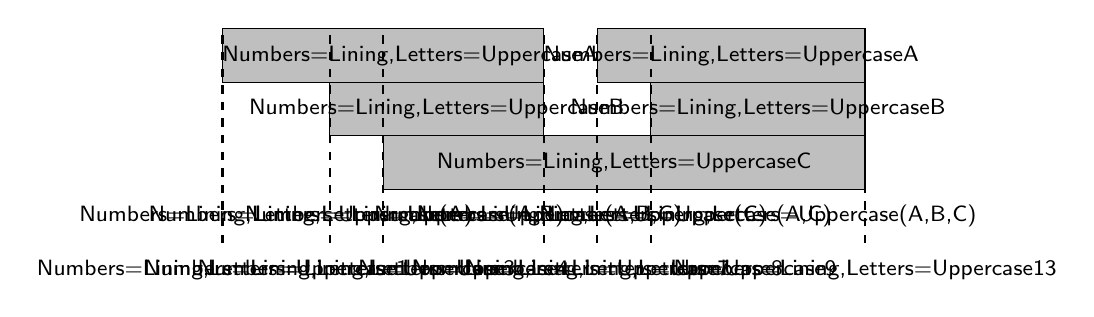
\begin{tikzpicture}[
	scale=0.68,
	every node/.append style={font=\footnotesize\sffamily\addfontfeature{Numbers=Lining,Letters=Uppercase}}]
	% boxes
	\draw [fill=lightgray] (0,4) rectangle (6,5);  % A1
	\node at (3.5,4.5) {A};
	
	\draw [fill=lightgray] (7,4) rectangle (12,5);  % A2
	\node at (9.5,4.5) {A};
	
	\draw [fill=lightgray] (2,3) rectangle (6,4);  % B1
	\node at (4,3.5) {B};
	
	\draw [fill=lightgray] (8,3) rectangle (12,4);  % B2
	\node at (10,3.5) {B};
	
	\draw [fill=lightgray] (3,2) rectangle (12,3);  % C
	\node at (7.5,2.5) {C};
	
	% item sets
	\node at (1,1.5) {(A)};
	\node at (2.5,1.5) {(A,B)};
	\node at (4.5,1.5) {(A,B,C)};
	\node at (6.5,1.5) {(C)};
	\node at (7.5,1.5) {(A,C)};
	\node at (10,1.5) {(A,B,C)};
	
	% time points
	\node at (0,0.5) {1};
	\node at (2,0.5) {3};
	\node at (3,0.5) {4};
	\node at (6,0.5) {7};
	\node at (7,0.5) {8};
	\node at (8,0.5) {9};
	\node at (12,0.5) {13};
	
	% time point lines
	\draw [dashed, thick] (0,1) -- (0,5);
	\draw [dashed, thick] (2,1) -- (2,5);
	\draw [dashed, thick] (3,1) -- (3,5);
	\draw [dashed, thick] (6,1) -- (6,5);
	\draw [dashed, thick] (7,1) -- (7,5);
	\draw [dashed, thick] (8,1) -- (8,5);
	\draw [dashed, thick] (12,1) -- (12,5);
	
	% text representation
%	\node at (6,0) {\code{<(A [1,3]),(A,B [3,4]),(A,B,C [4,7]),(C [7,9])(A,B,C [9,13])>}};
\end{tikzpicture}

\subsection{Mining Approach}
\label{sec:mining}
The fundamental aim of \fpmlower\ techniques is to find patterns in a data set that occur \emph{frequently}. The specific kind of pattern and the definition of \emph{frequent} cannot be generalised and depend heavily on the individual application. In contrast to descriptive and inferential statistics, which disprove or affirm hypotheses generated beforehand, \fpmlower\ is of an exploratory, hypothesis-generating nature. Depending on the patterns found, one may then formulate hypotheses afterwards, which may then in turn be tested empirically using descriptive and inferential statistics \cite[\pnum{6~ff.,~tba}]{rohlfing18,han12}.%% ISSUE: How do you give page references for each individual source when citing multiple sources?

\subsubsection{Association Rules}
The patterns \citet{rohlfing18} looked for were association rules of the form \fpmrule{A}{B}, where the probability of the succedent \fpmset{B} was high given the antecedent \fpmset{A}. Note that antecedent and succedent are not single events but sets of events. One may equally well form a hypothetical rule of the form \fpmrule{B,D}{A,C,D}. Occurrences of a rule were taken into account if they fulfilled one of two conditions:

\begin{enumerate}
	\item The antecedent's start time point lies before that of the succedent.
	\item The antecedent's and succedent's start time points are identical, i.e.\ they begin simultaneously.
\end{enumerate}

Referring again to Figure \ref{fig:idealseq}, one can for example observe the rules \fpmrule{A}{B} and \fpmrule{A}{B, C} (because the start time point of the antecedent lies before that of the succedent), but not \fpmrule{B}{A}.

This scheme can be further adapted to the specific nature of the data. Given that the data are hand-coded and that time points are stored with a precision of ±1~ms%IS THAT TRUE??
, the second condition will in all probability never be true. Regarding the first cnodition, the natural imprecision of coding by hand can lead to one annotation beginning before or after another essentially by pure chance, when in fact the two events begin \emph{at the same time.} The notion of \emph{at the same time} itself is problematic as well. Humans exhibit a certain reaction time to stimuli, which varies depending on the nature of the stimuli (SOURCE) but is always greater than 0~ms. It logically follows that if both mother and infant begin exhibiting a certain event \emph{at the same time,} then one event cannot be a reaction to the other because such a reaction would demand an appropriate reaction time. Therefore, an interpersonal rule, where both events begin at the same time, is the result of pure chance. Not only will it be a meaningless rule, but also an incorrect rule and\dash accordingly\dash should not be captured as a rule at all.

\paragraph{Choosing appropriate delays}
Human reaction time (henceforth \rt) varies depending on a vast variety of factors, among which are
intensity, modality, and complexity of the stimulus \citep{brebner80},
age and gender \citep{der06},
state of alertness \citep{appelle74},
handedness \citep{dane03},
and even personality traits \citep{stelmack93}.
Quite obviously, many of those traits cannot be determined for the subjects in the corpus used in the present thesis. However, those factors which are most relevant (namely age of the subject and modality of the stimulus) are both captured in the data\footnote{Exact age of the mothers is not known. The important fact is that they are all full-grown adults.} and relatively easy to account for. Regarding modality, variation is so small that it may safely be neglected. \citet[\pnum{9}]{brebner80} ascribe the variation to ``differences in the peripheral mechanisms rather than in the central processes'' and give average\footnote{I use the term \emph{average} wherever sources do not state whether the value in question is a mean, median, mode, or other measure of centrality.} \rt s of 8--10~ms for acoustic stimuli and 20--40~ms for visual stimuli to reach the central processes. The resulting difference of 10--32~ms is on a scale so small that considering it would unnecessarily complicate the analysis without giving adequate advantages. Regarding age, mean \rt\ lies  between 1002--1124~ms for infants of age 6--9 months (N~=~24) and between 289--318~ms for adults of age 19--26 years (N=11) \citep[\pnum{95}]{leibold02}.\footnote{Stimulus was a pure (i.e.~sine wave) tone of 1000~Hz with loudness ranging from 40--60~dB. No numerical values given. Converted from line chart using the Engauge Digitizer software \citep{mitchell02}. The loudness corresponds to average conversation loudness \citep[\pnum{32}]{goerne06}} This corresponds

A further adjustment must be made related to coders' imprecision. For intrapersonal rules only, simultaneous start time points of two events are meaningful. In order to capture them accordingly, intrapersonal events with a maximum delay of XX~ms are considered to begin simultaneously. 

\section{Results}

%\subsection{Association Rules}
%In the following, I will first lay out the type of association rule used by \citet{rohlfing18} and then explain how I modified this scheme to better fit the interactional, multimodal nature of the data. The basic sequence is structured as follows:
%\begin{quote}
%	\code{<(A [1,3]),(A,B [3,4]),(A,B,C [4,7]),(C [7,8]),(A,C [8,9]),(A,B,C [9,13])>}
%\end{quote}
%
%In traditional sequential pattern mining, the basic data type---called a sequence---is an ordered set of (unordered) item sets \citep[\pnum{588~ff.}]{han12}. Here, every item set in the sequence has an additional annotation marking the start and end time points between which the item set (that is, one specific occurrence of it) is contained in the data. Figure \ref{fig:idealseq} gives a graphical representation of this example sequence. Rules of the sort \fpmrule{A}{B} must fulfil one of two conditions:
%\begin{enumerate}
%	\item The antecedent's start time point lies before that of the succedent.
%	\item The antecedent's and succedent's start time points are identical, i.e.\ they begin simultaneously.
%\end{enumerate}
%Therefore, in the example sequence one can observe the rules \fpmrule{A}{A,B} but not \fpmrule{B}{A,B}. The following three modifications improve the scheme to better fit the data:
%
%\paragraph{Imprecision of hand-coded data}
%The second condition is problematic given the nature of the data. Every annotation has been hand-coded and with coding by hand comes imprecision. Given the fact that the time points' are precise up to one millisecond, there will in all likelihood not be any two annotations that begin at the exact same point. After examination of the source files (i.e.\ \textsc{elan} files) and consultation with the coders I have decided to allow for a \imprecisiondelay\ delay such that two annotations \(a\) and \(b\) are treated as beginning simultaneously iff their start time points \(s_a\) and \(s_b\) lie no further than 300ms apart (\(|s_a - s_b| < 300ms\)). This delay accounts for the coders' imprecision.
%
%\paragraph{Inter- and intrapersonal rules}
%Given the dyadic nature of the data it is necessary to distinguish between inter- and intrapersonal rules not only in rule evaluation but already in the mining process. Depending on various factors, the average human reaction time to an event lies between XXX and XXXms. %values? source?
%It follows that if both mother and child begin an event at the same time or with a delay below reaction time, then the cooccurrence is pure chance and should not be considered a pattern. Analogous to the maximum delay described in the previous paragraph, interpersonal sequences are only considered with a minimum delay of \reactiontime\ between the time start points.
% !TEX root = ../ba_scrreprt_master.tex
% @author Marcel Ruland (2018)

\newcommand{\hnaught}{\textit{H}\textsubscript{\addfontfeature{Numbers=Lining}0}}
\newcommand{\hone}{\textit{H}\textsubscript{\addfontfeature{Numbers=Lining}1}}


\chapter{\significance}
\label{ch:significance}
\chapterintro{Significance tests are one of the most widely used statistical tools in academic work of virtually all disciplines dealing with some sort of numerical data. As is the case with most widely used tools, the temptation to merely learn its application and neglect conceptual understanding is present. I will try and bypass this fallacy by devoting section \ref{sec:signat} to the concept of statistical significance. The following section \ref{sec:sigmet} describes the creation of a null hypothesis to establish a baseline against which to test for significance. Finally, section \ref{sec:sigres} discusses the results.}

\section{The Nature of Significance}
\label{sec:significancenature}

\begin{quote}\small\singlespacing
``We are inclined to think that as far as a particular hypothesis is concerned, no test based upon the theory of probability can by itself provide any valuable evidence of the truth or falsehood of that hypothesis. But we may look at the purpose of test from another view-point. Without hoping to know whether each separate hypothesis is true or false, we may search for rules to govern our behavior with regard to them, in following which we insure that, in the long run of experience, we shall not be too often wrong.''

~ \hfill \citep[\pnum{TBA}]{neyman33}
\end{quote}

\paragraph{Numerical vs applied significance} A certain kind of lens might have a positive effect on sight that is statistically significant. At the same time, this positive effect can be so small that humans are unable to perceive a difference. While this effect is undoubtedly significant numerically, no one would pay money for a lens whose effect they do not perceive. In that sense, significance alone must not be accepted blindly, because significance in turn is blind to effect size or scale \citep[\cnum{8}]{frost17}.

\section{Method}
\label{sec:significancemethod}
The crucial missing piece for establishing the significance of a rule is a base case\dash or base distribution, so to speak\dash against which to compare the rule's probability. In other words: while there obviously is a real distribution, we lack a null distribution for comparison. The methodological approach I take, therefore, is to create a null distribution, which then serves as a basis for the real rules' probabilities to be tested for significance. This is in some respects similar to\dash and certainly inspired by\dash \citet[\pnum{10~f.}]{abuzhaya17}.

We take one of the ten sequences in the corpus. For each of the 11 dimensions individually (cf.~table \ref{tab:events}), we shuffle the events with respect to their start points in time, but leave their duration untouched, i.e.~we leave the position of their time end points untouched \emph{with respect to their time start points.} We also do not add or remove any events. This process is done for all 11 dimensions. Figure \ref{fig:null} gives an example hereof. The top half of the figure is an excerpt of real data taken from a sequence in the corpus. We see three events of type \code{mother\_voc}, three shorter events of type \code{mother\_gaze\_infant}, one longer event of type \code{infant\_gaze\_mother}, etc.\footnote{The excerpt taken did not contain events of all 11 types, empty dimensions have simply been omitted in the graphic.} The bottom half of the figure shows a corresponding null distribution. Notice how \code{mother\_voc} still contains the same three events of the same length but in a different temporal order. The same is true for all other dimensions.

We now have a distribution of the sequence which contains the exact same events as the real distribution, but shuffled in their temporal order. In other words, the only thing that has changed is the temporal arrangement of the events \emph{with respect to one another.} We will call this a null distribution and create 100 of its kind. % Why 100? Why not more/less?
We go through the same process for all of the 10 sequences and end up having 1000 null distributions, with 100 each corresponding to a given sequence.

Finally, to evaluate a rule's significance we take the distribution of its probability in all of the 1000 null distributions, i.e.~we obtain a probability distribution with 1000 data points. We then test for significance at \(\alpha\)~=~0.05 using some test or another. % Is this distribution normal? Central limit theorem?

\begin{figure}
	\centering
	% !TEX root = ../ba_master.tex
% @author Marcel Ruland (2018)
\begin{tikzpicture}[
	node distance=0 and 0,  % y, x for fuck knows what reason
	every node/.append style={font=\footnotesize\sffamily\addfontfeature{Numbers=Lining,Letters=Uppercase}}]
%	\draw [help lines, dashed] (0,0) grid (13,7);
	
	% time line
	\node (twenty) at (3,-0.25) {20};
	\node [left=of twenty] {\textit{time (sec)}};
	\node at (4,-0.25) {21};
	\node at (5,-0.25) {22};
	\node at (6,-0.25) {23};
	\node at (7,-0.25) {24};
	\node at (8,-0.25) {25};
	\node at (9,-0.25) {26};
	\node at (10,-0.25) {27};
	\node at (11,-0.25) {28};
	\node at (12,-0.25) {29};
%	\node at (13,-0.25) {30};  % overfull hbox
	\draw [help lines, dashed] (3,3) -- (3,4);
	\draw [help lines, dashed] (4,0) -- (4,7);
	\draw [help lines, dashed] (5,0) -- (5,7);
	\draw [help lines, dashed] (6,0) -- (6,7);
	\draw [help lines, dashed] (7,0) -- (7,7);
	\draw [help lines, dashed] (8,0) -- (8,7);
	\draw [help lines, dashed] (9,0) -- (9,7);
	\draw [help lines, dashed] (10,0) -- (10,7);
	\draw [help lines, dashed] (11,0) -- (11,7);
	\draw [help lines, dashed] (12,0) -- (12,7);
	\draw [help lines, dashed] (13,3) -- (13,4);
	
	% top grid
	\draw (3,4) -- (3,7);
	\draw (13,4) -- (13,7);
	\draw (3,4) -- (13,4);
	\draw (3,4.5) -- (13,4.5);
	\draw (3,5) -- (13,5);
	\draw (3,5.5) -- (13,5.5);
	\draw (3,6) -- (13,6);
	\draw (3,6.5) -- (13,6.5);
	\draw (3,7) -- (13,7);
	
	% bottom grid
	\draw (3,0) -- (3,3);
	\draw (13,0) -- (13,3);
	\draw (3,0) -- (13,0);
	\draw (3,0.5) -- (13,0.5);
	\draw (3,1) -- (13,1);
	\draw (3,1.5) -- (13,1.5);
	\draw (3,2) -- (13,2);
	\draw (3,2.5) -- (13,2.5);
	\draw (3,3) -- (13,3);
	
	% top labels
	\node (mothervoctop) at (3,6.75) {};
	\node (mothergazeinfanttop) at (3,6.25) {};
	\node (mothergazeobjtop) at (3,5.75) {};
	\node (infantvoctop) at (3,5.25) {};
	\node (infantgazemothertop) at (3,4.75) {};
	\node (infantgazeobjtop) at (3,4.25) {};
	\node [left=of mothervoctop] {\code{mother\_voc}};
	\node [left=of mothergazeinfanttop] {\code{mother\_gaze\_infant}};
	\node [left=of mothergazeobjtop] {\code{mother\_gaze\_obj}};
	\node [left=of infantvoctop] {\code{infant\_voc}};
	\node [left=of infantgazemothertop] {\code{infant\_gaze\_mother}};
	\node [left=of infantgazeobjtop] {\code{infant\_gaze\_obj}};
	
	% bottom labels
	\node (mothervocbottom) at (3,2.75) {};
	\node (mothergazeinfantbottom) at (3,2.25) {};
	\node (mothergazeobjbottom) at (3,1.75) {};
	\node (infantvocbottom) at (3,1.25) {};
	\node (infantgazemotherbottom) at (3,0.75) {};
	\node (infantgazeobjbottom) at (3,0.25) {};
	\node [left=of mothervocbottom] {\code{mother\_voc}};
	\node [left=of mothergazeinfantbottom] {\code{mother\_gaze\_infant}};
	\node [left=of mothergazeobjbottom] {\code{mother\_gaze\_obj}};
	\node [left=of infantvocbottom] {\code{infant\_voc}};
	\node [left=of infantgazemotherbottom] {\code{infant\_gaze\_mother}};
	\node [left=of infantgazeobjbottom] {\code{infant\_gaze\_obj}};
	
	% top annotations
	\draw [fill=lightgray] (3,6.5) rectangle (8.279,7);
	\draw [fill=lightgray] (8.279,6.5) rectangle (10.206,7);
	\draw [fill=lightgray] (10.206,6.5) rectangle (11.76,7);

	\draw [fill=lightgray] (6.96,6) rectangle (7.32,6.5);
	\draw [fill=lightgray] (10.28,6) rectangle (10.52,6.5);
	\draw [fill=lightgray] (12.68,6) rectangle (13,6.5);
	
	\draw [fill=lightgray] (3.84,5.5) rectangle (6.92,6);
	\draw [fill=lightgray] (7.36,5.5) rectangle (10.24,6);
	\draw [fill=lightgray] (10.56,5.5) rectangle (12.64,6);
	
	\draw [fill=lightgray] (3.887,5) rectangle (4.624,5.5);
	\draw [fill=lightgray] (6.74,5) rectangle (7.53,5.5);
	\draw [fill=lightgray] (8.279,5) rectangle (9.909,5.5);
	
	\draw [fill=lightgray] (3,4.5) rectangle (10.52,5);

	\draw [fill=lightgray] (10.56,4) rectangle (13,4.5);

	% bottom annotations
	\draw [fill=lightgray] (7.592,2.5) rectangle (12.871,3);
	\draw [fill=lightgray] (5.264,2.5) rectangle (7.191,3);
	\draw [fill=lightgray] (3.221,2.5) rectangle (4.775,3);

	\draw [fill=lightgray] (12.069,2) rectangle (12.429,2.5);
	\draw [fill=lightgray] (4.039,2) rectangle (4.279,2.5);
	\draw [fill=lightgray] (9.115,2) rectangle (9.435,2.5);
	
	\draw [fill=lightgray] (4.04,1.5) rectangle (7.12,2);
	\draw [fill=lightgray] (9.76,1.5) rectangle (12.64,2);
	\draw [fill=lightgray] (7.59,1.5) rectangle (9.64,2);
	
	\draw [fill=lightgray] (7.287,1) rectangle (8.024,1.5);
	\draw [fill=lightgray] (10.84,1) rectangle (11.63,1.5);
	\draw [fill=lightgray] (3.55,1) rectangle (5.18,1.5);
	
	\draw [fill=lightgray] (3.27,0.5) rectangle (10.79,1);

	\draw [fill=lightgray] (7.42,0) rectangle (9.86,0.5);
\end{tikzpicture}
	\caption{An excerpt of a real sequence (top) and a corresponding null distribution (bottom). Note how events are shuffled with respect to their position in time, whereas their duration and number has been left untouched.}
	\label{fig:null}
\end{figure}

%Tests to be used:
%- some sort of significance test
%- support(X->Y) = P(XUY) and confidence(X->Y) = P(Y|X), both associated with an \emph{arbitrary} cutoff threshold \citep[\pnum{21~ff.}]{han12}
%
%``[M]any patterns that are interesting by objective standards may represent common sense and, therefore, are actually uninteresting.'' \citep[\pnum{22}]{han12}

\section{Results}
\label{sec:significanceresults}
show and discuss significant rules
% !TEX root = ../ba_master.tex
% @author Marcel Ruland (2018)

\chapter{Visualising Significant Patterns}
\label{ch:visualisation}
\emph{chapter description goes here}

\section{Identifying the Challenge}
\label{sec:visualisationchallenge}
Which questions should be answered in an instant? Which information is vital, which information is neglectable and why?

\section{Ways of Evaluating Visualisations}
\label{sec:visualisationevaluation}
several metrics from \citepos{cairo13} books. Which values should our visualisation have?

\section{Proposing a Visualisation} % so so so much a working title omg I can't even
\label{sec:visualisationproposal}
this is where the actual visualisation is introduced and explained

% !TEX root = ../ba_master.tex
% @author Marcel Ruland (2018)

\chapter{Conclusion}
\label{ch:conclusion}
%formulate some hypotheses from the results
\appendix
% !TEX root = ../ba_scrreprt_master.tex
% @author Marcel Ruland (2018)

\chapter{Formalisation of Association Rules}
\label{ch:formalisation}

The rules mined are of the form \fpmrule{A}{B}, where \fpmset{A} is the antecedent (or condition that must be fulfilled) and \fpmset{B} is the succedent (or result given the antecedent).
Both antecedent and succedent are sets of events, where an event is one of those listed in table \ref{tab:events}.
Events may be of the type \code{mother} or \code{infant}.
Stored with every set of events is the time start and end point of the interval during which the set is observed in the data.
The example sequence given in figure \ref{fig:idealseq} contains 6 different such intervals.
An occurrence of a rule must fulfil one of the following conditions in order to be taken into account:
\begin{enumerate}
	\item If the antecedent is of type \code{infant} and the succedent of type \code{mother}, then the succedent's start time point must lie at least 289~ms after the start time point of the antecedent and the end time point of the antecedent must lie after the start time point of the succedent.
	\item If the antecedent is of type \code{mother} and the succedent of type \code{infant}, then the succedent's start time point must lie at least 850~ms after the start time point of the antecedent and the end time point of the antecedent must lie after the start time point of the succedent.
	\item If both antecedent and succedent are of the same type, then the succedent's start time point must lie no more than 40~ms before the start time point of the antecedent and the end time point of the antecedent must lie after the start time point of the succedent.
\end{enumerate}
From the third condition follows, that if a rule \fpmrule{A}{B} fulfils it and the start time point \fpmset{A} of the rule lies less than 40~ms before the start time point of the succedent \fpmset{B} of the rule, then it also counts as an occurrence of the rule \fpmrule{B}{A}.

\listoftables
\listoffigures
\KOMAoptions{fontsize=8pt}
\bibliography{../aux/bib/BA_Marcel}

\end{document}
